\documentclass[10pt,twocolumn,a4paper]{article}

\usepackage[top=1.35cm, bottom=1.35cm, left=1.35cm, right=1.35cm]{geometry}
\usepackage{amsmath,amssymb}
\usepackage{graphicx}
\usepackage{booktabs}
\usepackage{microtype}
\usepackage{hyperref}
\usepackage{xcolor}
\usepackage{caption}
\usepackage{subcaption}
\usepackage{enumitem}
\usepackage{titlesec}

% Search both local directory and results/figures/
\graphicspath{{results/figures/}{./}}

% Hyperlink setup
\hypersetup{
    colorlinks=true,
    linkcolor=blue!70!black,
    citecolor=blue!70!black,
    urlcolor=blue!70!black
}

% Tight spacing for conference-style report layout
\titlespacing*{\section}{0pt}{3.5pt}{1.5pt}
\titlespacing*{\subsection}{0pt}{2.5pt}{1.0pt}
\titlespacing*{\subsubsection}{0pt}{1.8pt}{0.8pt}
\setlength{\parskip}{1.2pt}
\setlength{\parindent}{0pt}

% Float and caption spacing adjustments to fit strictly within 5 pages
\setlength{\textfloatsep}{3.5pt plus 1pt minus 1pt}
\setlength{\floatsep}{3.5pt plus 1pt minus 1pt}
\setlength{\intextsep}{3.5pt plus 1pt minus 1pt}
\setlength{\abovecaptionskip}{2pt}
\setlength{\belowcaptionskip}{1pt}
\setlist{nosep, topsep=0.5pt, parsep=0pt, partopsep=0pt, itemsep=0.5pt, leftmargin=*}

\title{\textbf{\Large Benchmarking Approximate Nearest Neighbour Search:\\Trade-offs in Space Partitioning, Proximity Graphs, and Quantization}}
\author{%
  \textbf{G Sai Sri Harsha} \quad \textbf{Roll No.:} 2024101034 \\
  \textit{CS4.406: Information Retrieval \& Extraction (Monsoon 2026)} \\
  International Institute of Information Technology, Hyderabad
}
\date{\vspace{-1.5em}}

\begin{document}

\maketitle

\begin{abstract}
Dense vector retrieval relies critically on Approximate Nearest Neighbour (ANN) search to overcome the linear scaling bottleneck of exact brute force comparison. In this work, we present an end-to-end empirical benchmark of three dominant ANN index paradigms---Hierarchical Navigable Small World graphs (HNSW), Inverted File with Flat storage (IVF-Flat), and Inverted File with Product Quantization (IVF-PQ)---against exact search across standard benchmarks (SIFT-128 and GloVe-100) and custom synthetic datasets. We evaluate throughput (QPS), recall@10 with exact boundary tie-breaking, build overhead, and memory footprint. We demonstrate that while HNSW achieves highest peak throughput on clustered image descriptors (7,458 QPS measured, 8,278 QPS interpolated at 0.95 recall on SIFT), its advantage shrinks to only $1.24\times$ over IVF-Flat on dense word embeddings (GloVe) due to high intrinsic dimensionality and hubness. Furthermore, we investigate the fundamental recall ceiling of plain IVF-PQ, proving that sub-space quantization distortion is the root cause and that exact re-ranking of the top-100 candidates completely restores recall to $>0.96$ at 3,664.4 QPS ($87\times$ faster than exact search) while retaining memory savings. Finally, using a parameterized synthetic Gaussian mixture generator ($N=200\text{K}, D=64$), we expose the catastrophic failure mode of space-partitioning under cluster dispersion, where Voronoi boundary scattering causes IVF-Flat recall to drop by $23.8\%$ and prevents both indexes from reaching 0.95 recall.
\end{abstract}

\section{Introduction \& Exact Baseline (Part 1)}
Finding the $k$ nearest stored vectors to a query $\mathbf{q} \in \mathbb{R}^D$ is the core operational primitive of dense information retrieval. Formally, given a dataset $\mathcal{X} = \{\mathbf{x}_1, \dots, \mathbf{x}_N\} \subset \mathbb{R}^D$, exact search evaluates the Euclidean distance $\|\mathbf{q} - \mathbf{x}_i\|_2$ across all $N$ vectors, sorting the resulting distances in $\mathcal{O}(ND + N \log k)$ time. At web scale ($N \ge 10^7$), exhaustive comparison exceeds latency budgets, requiring ANN indexing structures that sacrifice perfect recall for orders-of-magnitude throughput gains.

\subsection{Benchmark Environment \& Specifications}
All experiments were conducted on a single dedicated machine to maintain measurement consistency:
\begin{itemize}
    \item \textbf{CPU}: 12th Gen Intel Core i5-12450HX (8 cores, 12 threads, base clock 2.4 GHz, up to 4.4 GHz Turbo, 12 MB L3 cache).
    \item \textbf{Memory}: 12 GB DDR4 RAM (11.5 GiB usable), 8.0 GB Swap.
    \item \textbf{Operating System}: Fedora Linux 44 (Kernel 7.2.11-200.fc44.x86\_64, glibc 2.43).
    \item \textbf{Software Stack}: Python 3.14.8, FAISS-CPU 1.15.1, NumPy 2.5.4, SciPy 1.18.1, Matplotlib 3.11.2.
    \item \textbf{Measurement Protocol}: Single-thread execution enforced via \texttt{faiss.omp\_set\_num\_threads(1)}. Latency and QPS are reported as the median of 3 independent runs over test queries (last 5,000 queries of the standard 10,000 query sets).
\end{itemize}

\subsection{Exact Baseline \& Metric Agreement}
We implemented exact brute-force search using \texttt{faiss.IndexFlatL2}. Ground-truth nearest neighbours and squared $L_2$ distances provided in the HDF5 datasets were compared against our exact baseline. To prevent counting equidistant candidates as errors, we implemented a custom tie-aware \texttt{recall@10} function:
\begin{equation}
\text{Recall@}k(\mathcal{I}_q, \mathcal{G}_q) = \frac{1}{k} \sum_{i=1}^k \mathbf{1}\Big( \mathbf{x}_{\mathcal{I}_q[i]} \in \mathcal{G}_q \;\lor\; d(\mathbf{q}, \mathbf{x}_{\mathcal{I}_q[i]}) \le d_k^* + \epsilon \Big)
\end{equation}
where $d_k^*$ is the distance to the $k$-th ground-truth neighbour and $\epsilon = 10^{-5}$. The exact search results achieved an exact agreement of $1.000000$ on both SIFT-128 and GloVe-100.

\begin{table}[t]
\centering
\small
\caption{Exact Search Baseline (\texttt{IndexFlatL2}) Performance}
\label{tab:exact_baseline}
\resizebox{\columnwidth}{!}{%
\begin{tabular}{lccccc}
\toprule
\textbf{Dataset} & \textbf{Build (s)} & \textbf{RAM} & \textbf{1-by-1 QPS} & \textbf{Batch QPS} & \textbf{Speedup} \\
\midrule
SIFT-128  & 0.22s & 488 MB & 42.2 & 313.1 & \textbf{7.43$\times$} \\
GloVe-100 & 0.20s & 451 MB & 45.7 & 315.6 & \textbf{6.91$\times$} \\
\bottomrule
\end{tabular}%
}
\end{table}

\subsection{The Batch vs. Single-Query Speedup Mechanism}
As summarized in Table~\ref{tab:exact_baseline}, evaluating queries in a single matrix batch yields a \textbf{7.43$\times$ speedup on SIFT} (313.1 QPS vs. 42.2 QPS) and \textbf{6.91$\times$ on GloVe} (315.6 QPS vs. 45.7 QPS). This disparity is governed by three architectural mechanisms:
\begin{enumerate}
    \item \textbf{Level-3 vs. Level-2 BLAS}: Batch search computes $\|\mathbf{Q} - \mathbf{X}\|^2 = \operatorname{diag}(\mathbf{Q}\mathbf{Q}^T) + \operatorname{diag}(\mathbf{X}\mathbf{X}^T) - 2\mathbf{Q}\mathbf{X}^T$. The matrix product $\mathbf{Q}\mathbf{X}^T$ leverages Level-3 BLAS (\texttt{SGEMM}), achieving high arithmetic intensity through register tiling, loop unrolling, and AVX2 SIMD fusions. In contrast, sequential single-query search evaluates matrix-vector products (\texttt{SGEMV}, Level-2 BLAS), where one vector operand is read per floating-point operation, rendering the computation entirely memory-bandwidth bound.
    \item \textbf{Cache Locality \& Memory Bus Traffic}: For 5,000 queries, batch search amortizes each L2/L3 cache-line read across all queries. Sequential search forces the CPU to stream the entire 488~MB base dataset from main memory for \textit{every single query}, generating $5,000 \times 488\text{ MB} \approx 2.44\text{ TB}$ of memory traffic across the memory controller, incurring severe cache misses and memory bus saturation.
    \item \textbf{Instruction \& Thread Synchronization Overhead}: Single-query loops incur 5,000 separate function calls, stack allocations, and OpenMP thread dispatch synchronizations, whereas batch execution invokes the compute kernel in a single call.
\end{enumerate}

\section{Benchmarking Three ANN Indexes (Part 2)}
We evaluated three established ANN index families:
\begin{itemize}
    \item \textbf{HNSW} (\texttt{IndexHNSWFlat}): Multi-layer proximity graph with Delaunay-like greedy routing. Build parameters: $M \in \{16, 32\}$, $efConstruction = 64$. Search parameter: $efSearch \in [10, 1200]$.
    \item \textbf{IVF-Flat} (\texttt{IndexIVFFlat}): Inverted file with $k$-means Voronoi partitioning. Build parameter: $nlist \in \{1024, 2048, 4096\}$. Search parameter: $nprobe \in [1, 512]$.
    \item \textbf{IVF-PQ} (\texttt{IndexIVFPQ}): Inverted file with Product Quantization codes ($m=16$, $nbits=8$). Search parameter: $nprobe \in [1, 256]$.
\end{itemize}

\begin{figure*}[t]
    \centering
    \begin{subfigure}[b]{0.49\textwidth}
        \centering
        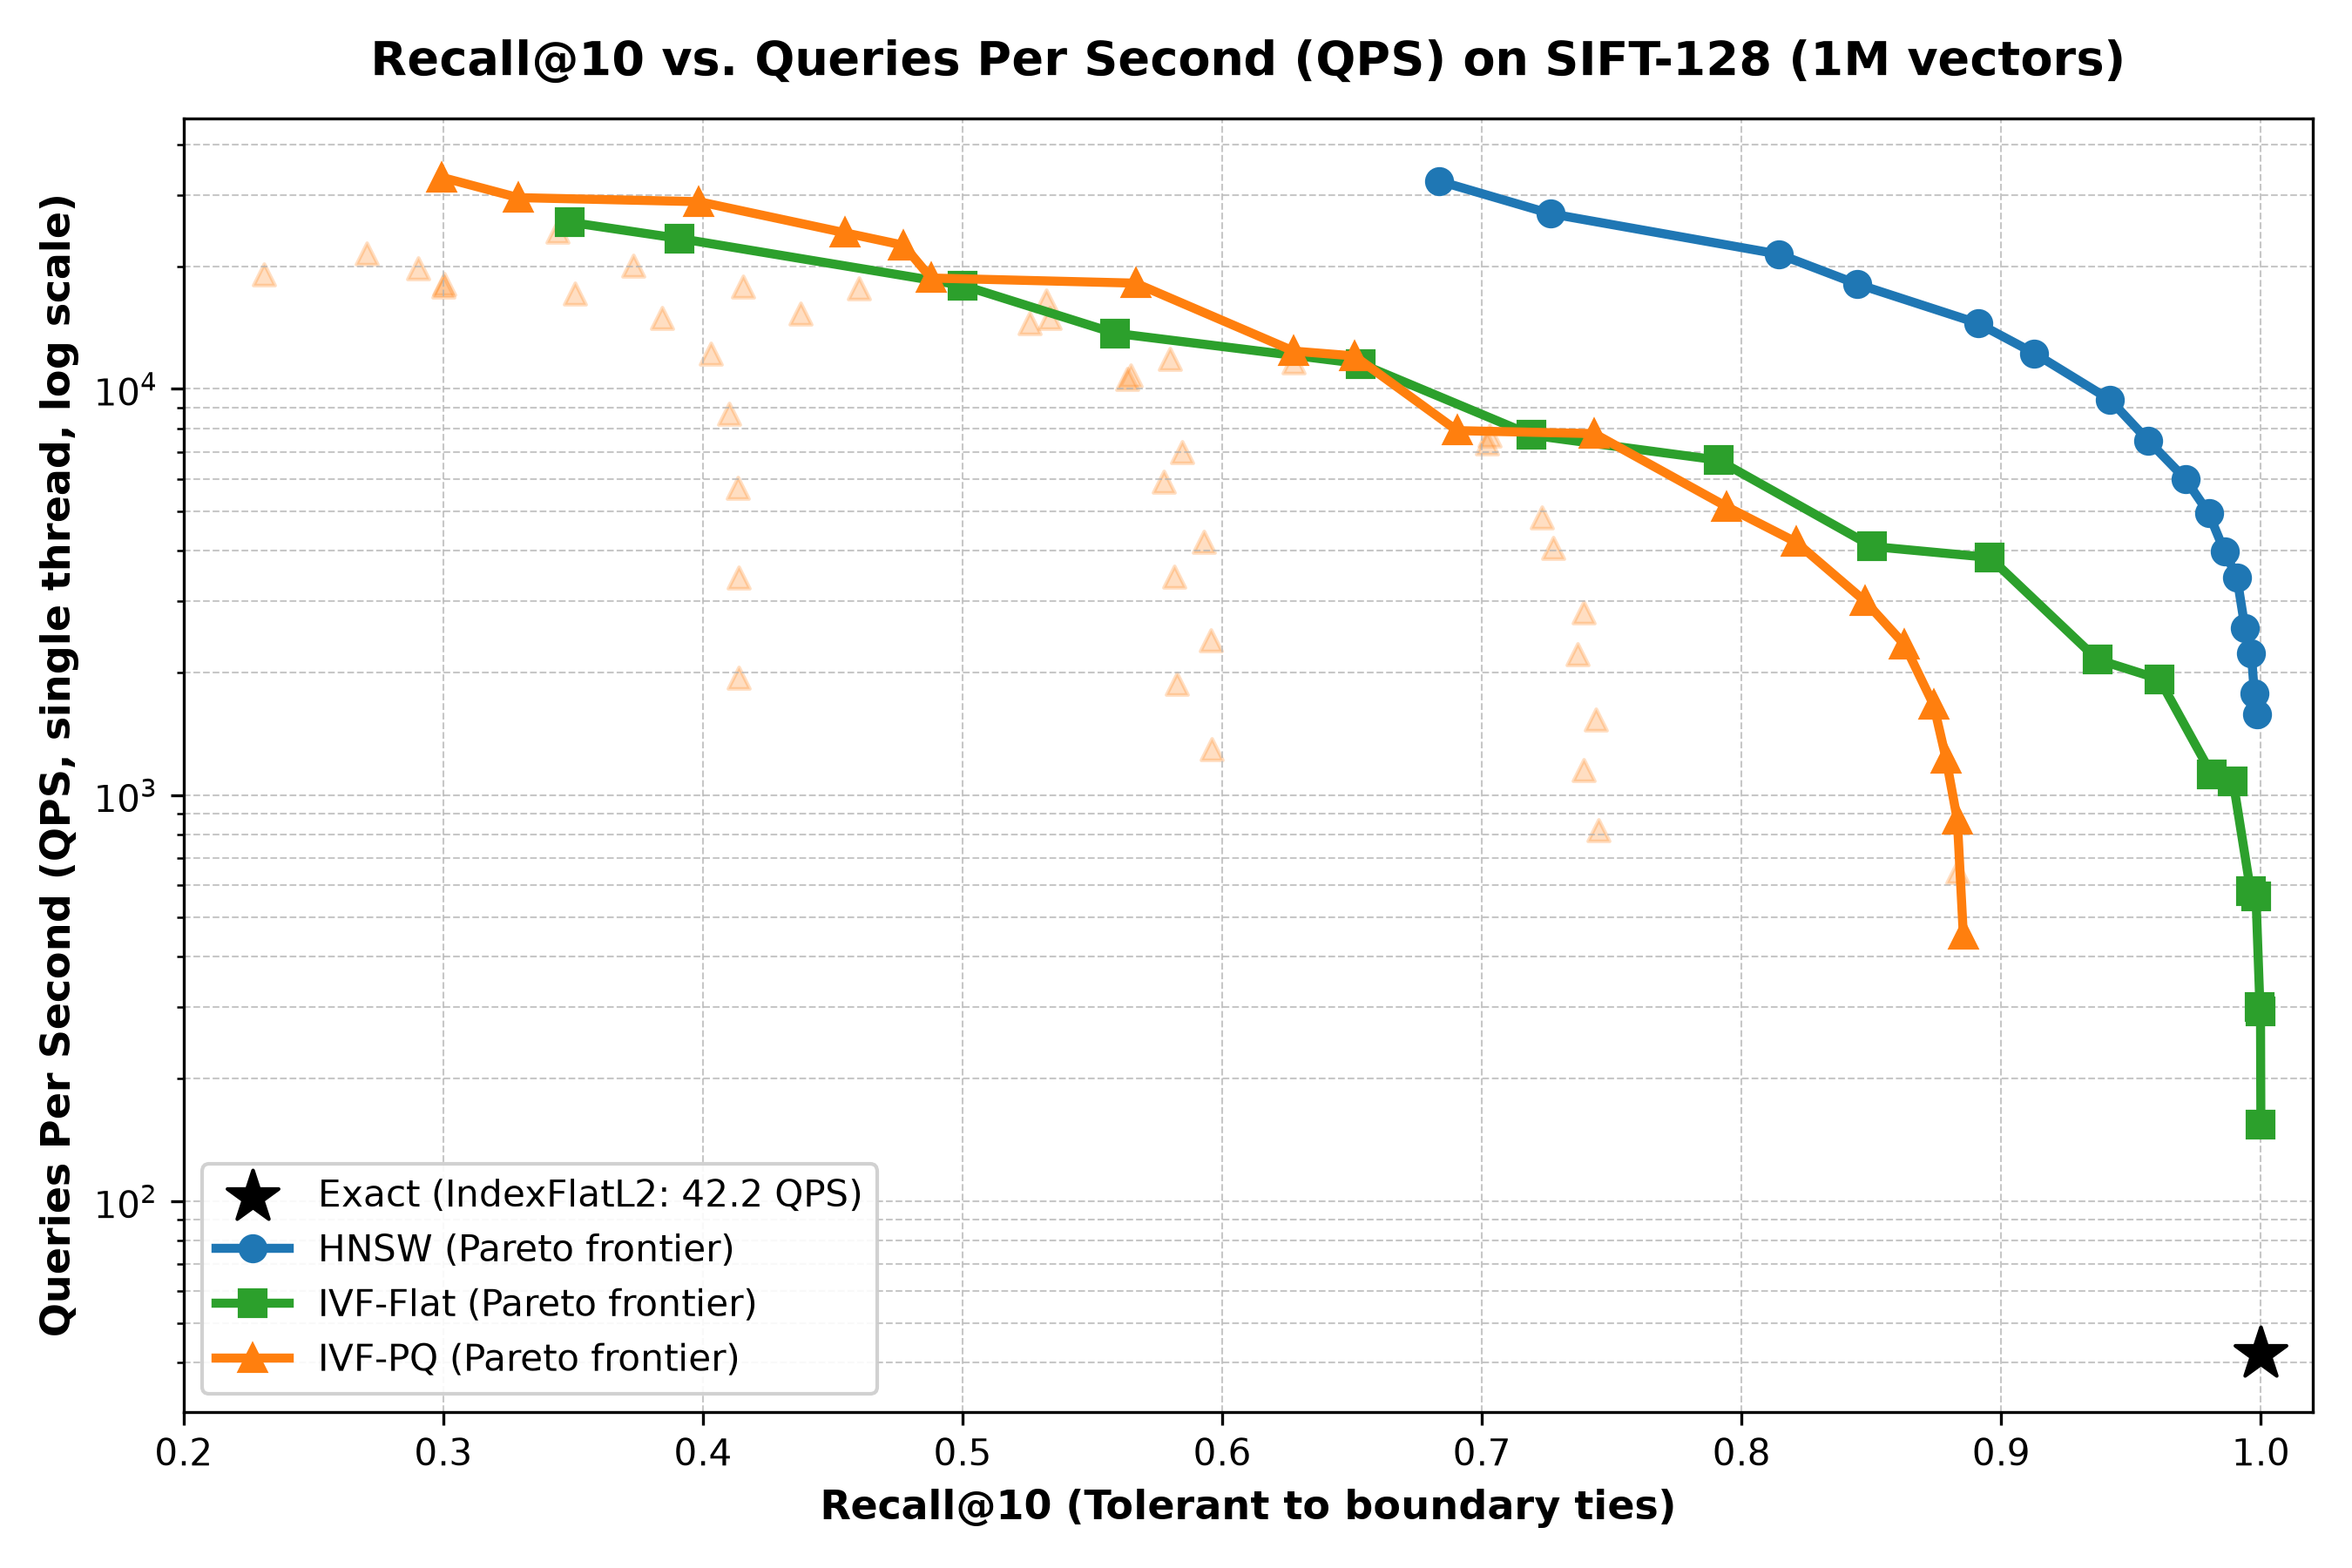
\includegraphics[width=\linewidth, height=3.6cm]{part2_sift_tradeoff.png}
        \caption{SIFT-128 (1M vectors, 128 dimensions, Euclidean)}
        \label{fig:part2_sift}
    \end{subfigure}\hfill
    \begin{subfigure}[b]{0.49\textwidth}
        \centering
        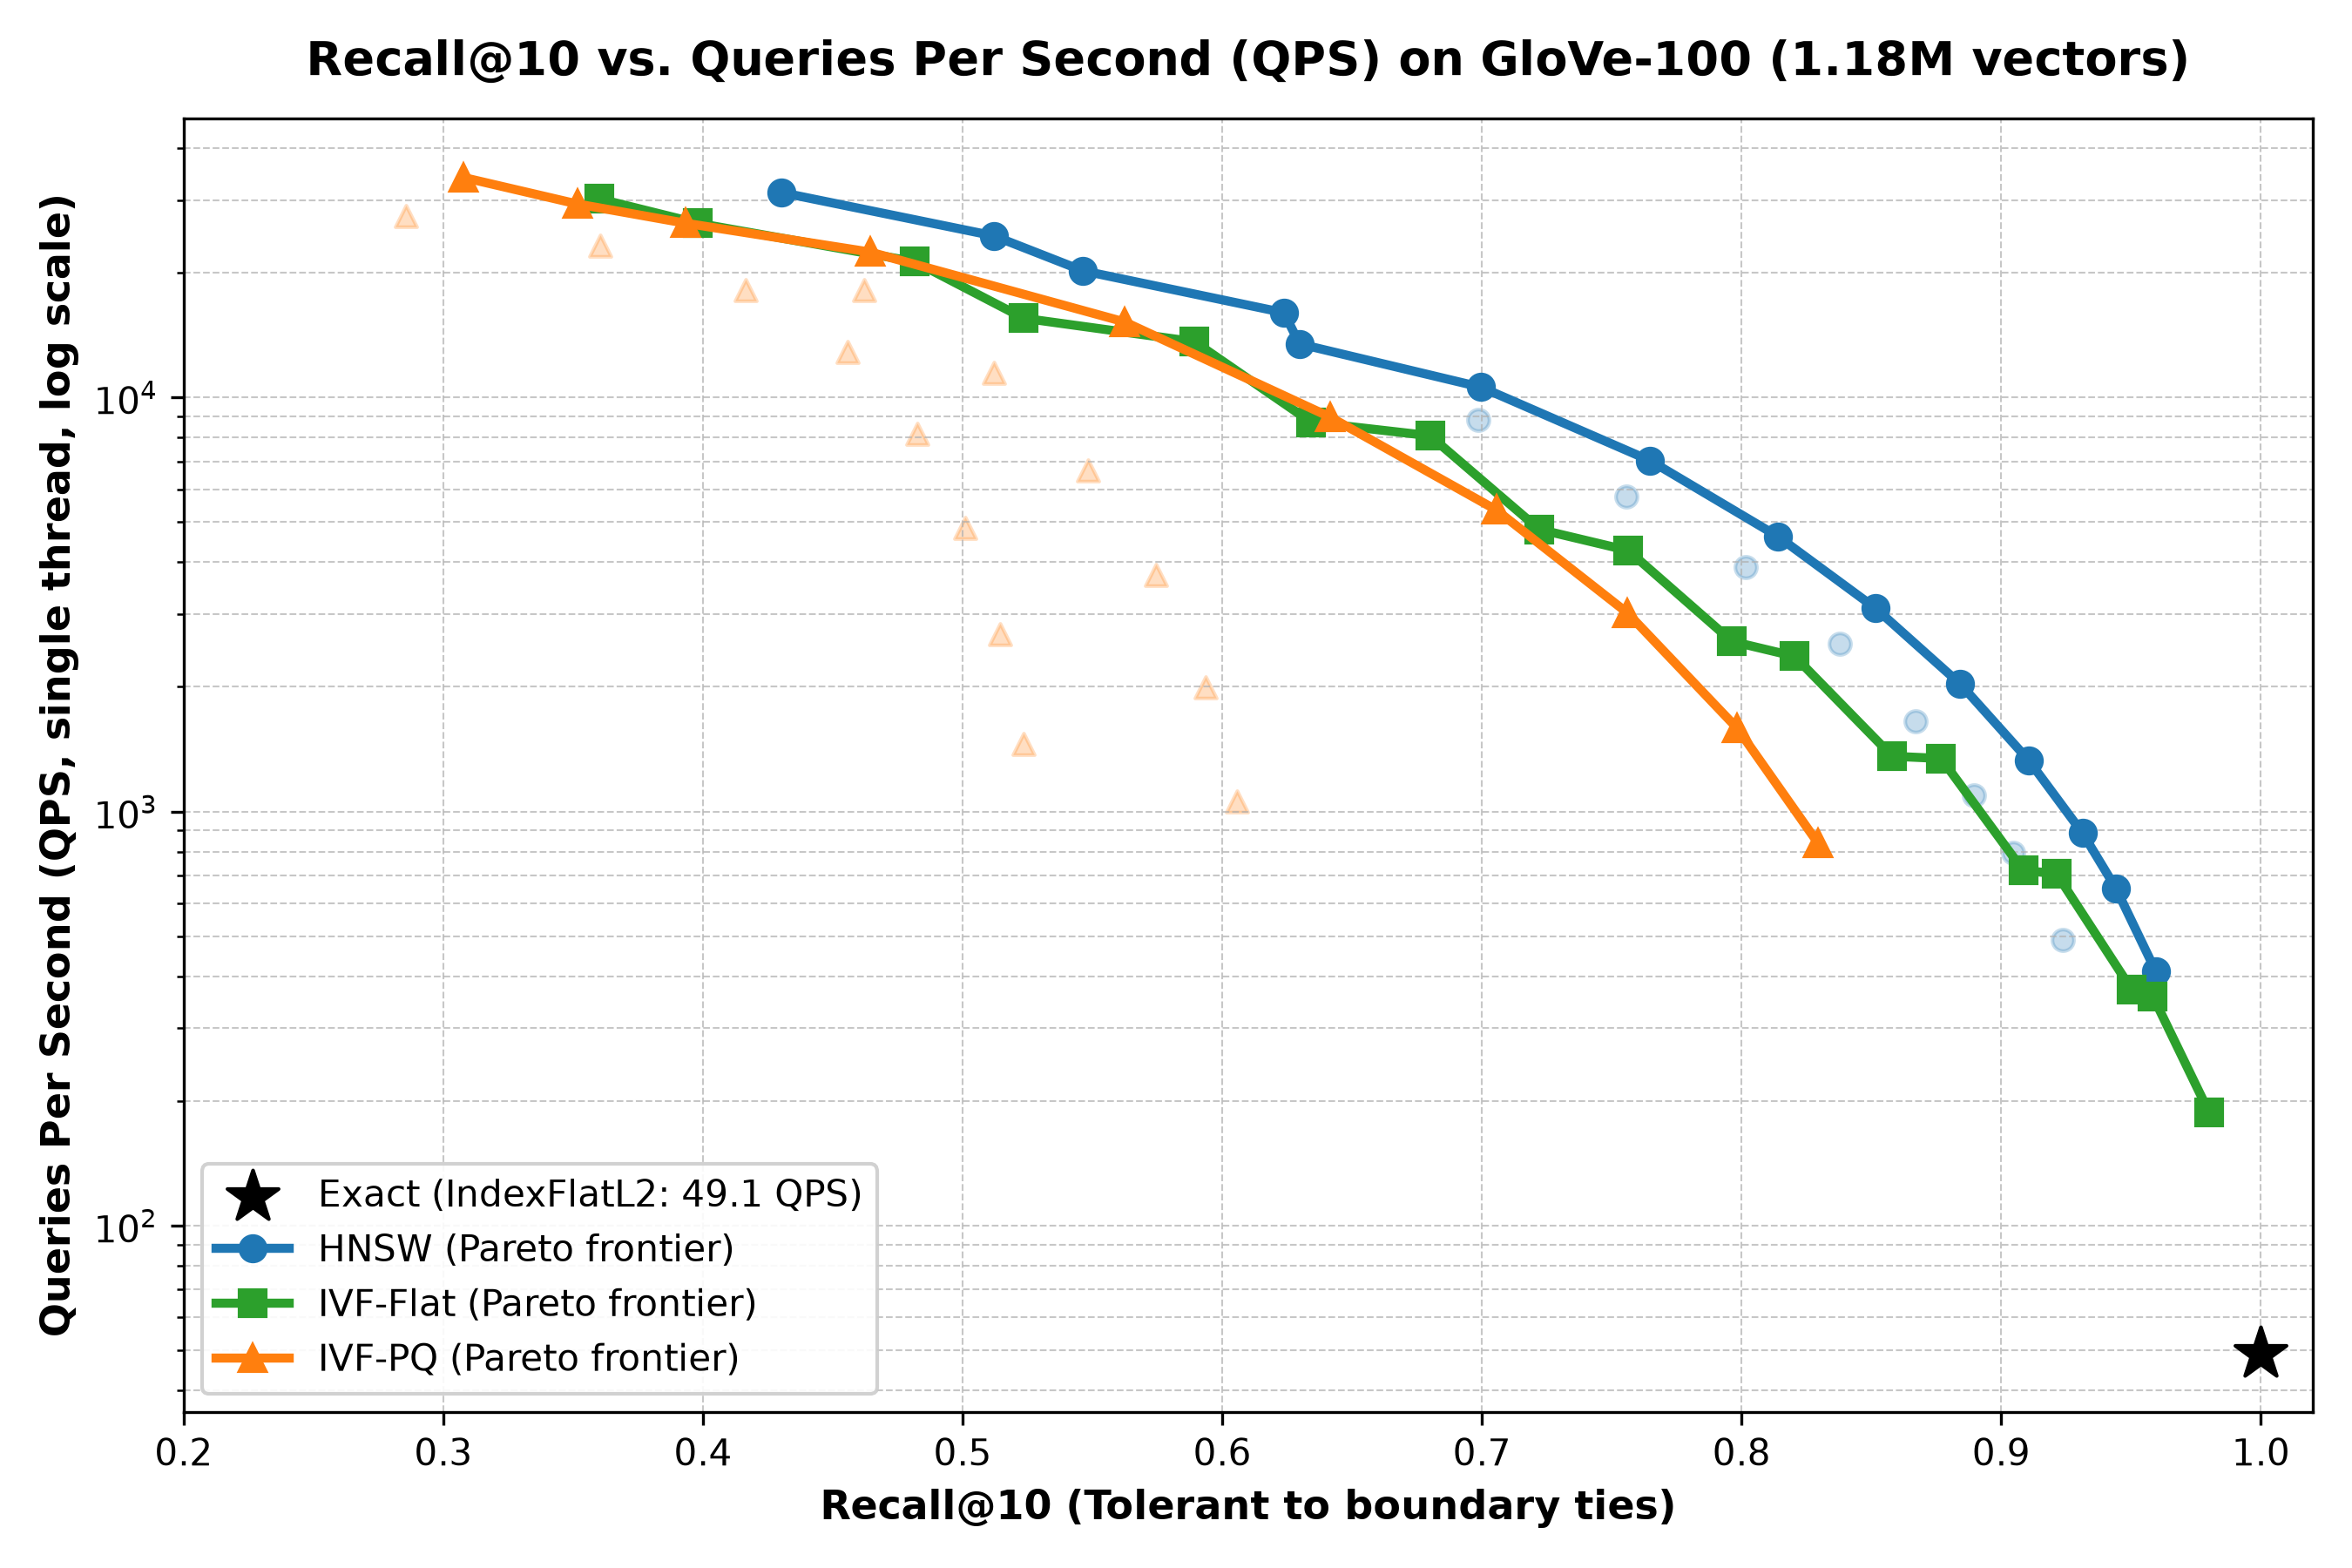
\includegraphics[width=\linewidth, height=3.6cm]{part2_glove_tradeoff.png}
        \caption{GloVe-100 (1.18M vectors, 100 dimensions, Angular)}
        \label{fig:part2_glove}
    \end{subfigure}
    \caption{Recall@10 vs. single-query QPS trade-off curves for HNSW, IVF-Flat, and IVF-PQ against the exact baseline.}
    \label{fig:part2_tradeoffs}
\end{figure*}

\subsection{Performance at High-Recall Targets}
Figure~\ref{fig:part2_tradeoffs} shows the Pareto frontiers for both datasets. The throughput numbers at standard operational targets (Recall = 0.90 and 0.95) are summarized in Table~\ref{tab:part2_qps}.

\begin{table}[t]
\centering
\small
\caption{Queries Per Second (QPS) at Recall Targets (Part 2)}
\label{tab:part2_qps}
\resizebox{\columnwidth}{!}{%
\begin{tabular}{lcccc}
\toprule
& \multicolumn{2}{c}{\textbf{SIFT-128}} & \multicolumn{2}{c}{\textbf{GloVe-100}} \\
\cmidrule(lr){2-3} \cmidrule(lr){4-5}
\textbf{Index Type} & \textbf{@ 0.90} & \textbf{@ 0.95} & \textbf{@ 0.90} & \textbf{@ 0.95} \\
\midrule
\textbf{HNSW}          & 13,528.9 & \textbf{7,457.6} & 1,419.9 & \textbf{446.0} \\
\textbf{IVF-Flat}      &  3,616.5 & 2,030.0          &   940.2 & 359.2 \\
\textbf{IVF-PQ} ($m=16$) & N/A      & N/A (max 0.885)  & N/A     & N/A (max 0.829) \\
\textbf{Exact Brute}   &    42.2 &    42.2          &    45.7 &   45.7 \\
\bottomrule
\end{tabular}%
}
\end{table}

\subsection{Resource Footprint at Recall 0.95}
Table~\ref{tab:part2_resources} presents the build time, serialized index size, and effective bytes per vector at the target operating point ($R \ge 0.95$).

\begin{table}[t]
\centering
\small
\caption{Resource Footprint at Recall 0.95 (or Maximum Achieved)}
\label{tab:part2_resources}
\resizebox{\columnwidth}{!}{%
\begin{tabular}{lcccc}
\toprule
\textbf{Index} & \textbf{Build (s)} & \textbf{Size (MB)} & \textbf{Bytes/Vec} & \textbf{Recall} \\
\midrule
\multicolumn{5}{l}{\textit{\textbf{SIFT-128} (1,000,000 vectors, 128-d, raw = 512 B/vec)}} \\
HNSW ($M=32$)           & 130.63s & 747.8 MB & 784.1 B & 0.9566 \\
IVF-Flat ($nlist=2048$) &  37.60s & 496.9 MB & 521.1 B & 0.9609 \\
IVF-PQ ($m=16$)         &  48.15s &  70.8 MB &  74.3 B & 0.8851 (Ceil.) \\
Exact                   &   0.22s & 488.3 MB & 512.0 B & 1.0000 \\
\midrule
\multicolumn{5}{l}{\textit{\textbf{GloVe-100} (1,183,514 vectors, 100-d, raw = 400 B/vec)}} \\
HNSW ($M=32$)           & 208.27s & 758.6 MB & 672.2 B & 0.9597 \\
IVF-Flat ($nlist=2048$) &  33.97s & 460.9 MB & 408.4 B & 0.9585 \\
IVF-PQ ($m=20$)         &  42.31s &  66.4 MB &  58.8 B & 0.8291 (Ceil.) \\
Exact                   &   0.20s & 451.5 MB & 400.0 B & 1.0000 \\
\bottomrule
\end{tabular}%
}
\end{table}

\subsection{Why Plain IVF-PQ Fails to Reach High Recall}
A primary observation across both datasets is that plain IVF-PQ hits an impassable recall ceiling: \textbf{0.885 on SIFT} and \textbf{0.829 on GloVe}, failing to achieve 0.90 or 0.95 recall regardless of the search budget ($nprobe \le 512$). 

The mechanism behind this failure is \textbf{irreducible quantization distortion}. Product Quantization decomposes $\mathbb{R}^D$ into $m$ orthogonal sub-spaces $\mathbb{R}^{D/m}$, quantizing each sub-vector $\mathbf{x}^{(j)}$ to its nearest centroid $\mathbf{c}_k^{(j)}$ from a codebook of size $k^* = 256$ ($8$ bits). During asymmetric distance computation (ADC):
\begin{equation}
\tilde{d}(\mathbf{q}, \mathbf{x})^2 = \sum_{j=1}^m \|\mathbf{q}^{(j)} - \mathbf{c}_{i_j}^{(j)}\|_2^2 = d(\mathbf{q}, \mathbf{x})^2 + \epsilon_{ADC}
\end{equation}
The distance error $\epsilon_{ADC}$ introduces rank noise. Even when inverted lists successfully retrieve the true 10-NN candidates into the candidate buffer, the quantized distance approximations perturb the relative ordering among closely spaced candidates. Because the gap between the 10th and 50th true neighbour is frequently smaller than $\epsilon_{ADC}$, true nearest neighbours are displaced outside the top-10. Increasing $nprobe$ scans more Voronoi cells and adds more candidates, but cannot resolve sub-space distance noise.

\section{Standard Data Experiment: Compression \& Exact Re-ranking (Part 3)}
To address the recall ceiling observed in Part 2, we conducted the Part 3 Compression Experiment on SIFT-128. Prior to running the experiment, our formal hypotheses were registered and committed in git (\texttt{commit 36d726d}).

\begin{figure*}[t]
    \centering
    \begin{subfigure}[b]{0.49\textwidth}
        \centering
        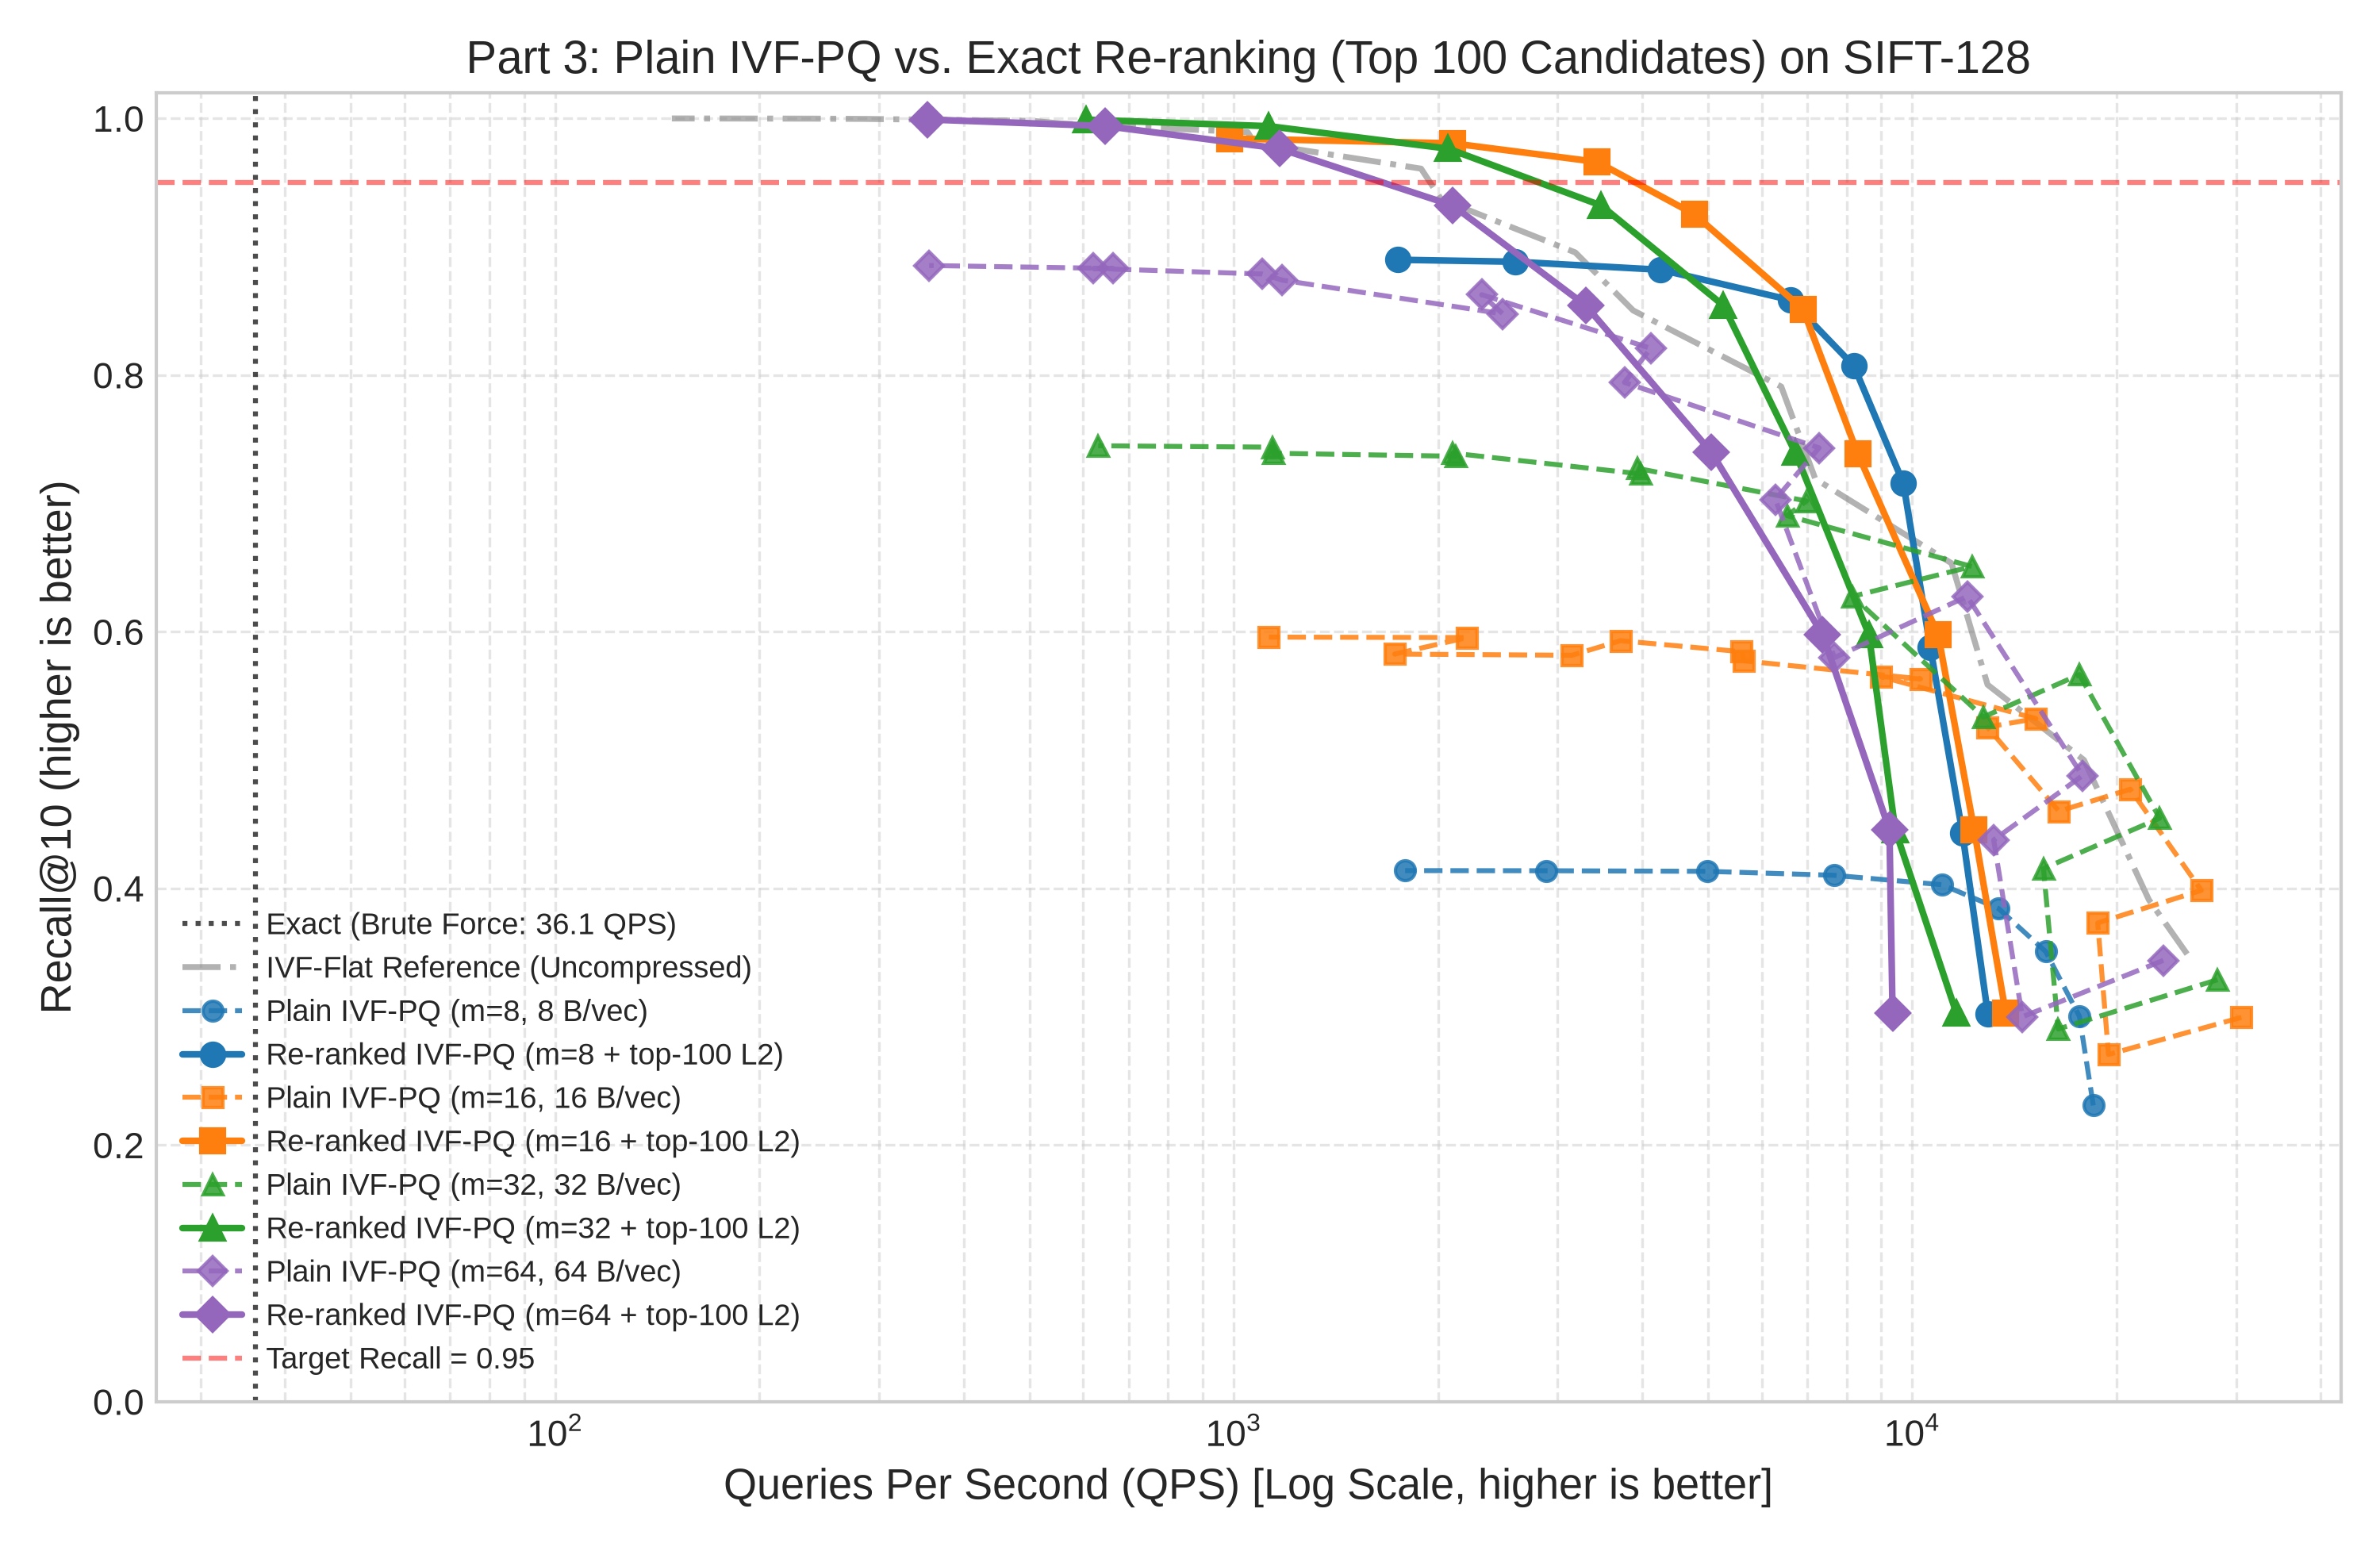
\includegraphics[width=\linewidth, height=3.6cm]{part3_compression_tradeoff.png}
        \caption{Recall@10 vs. QPS trade-off curves}
        \label{fig:part3_tradeoff}
    \end{subfigure}\hfill
    \begin{subfigure}[b]{0.49\textwidth}
        \centering
        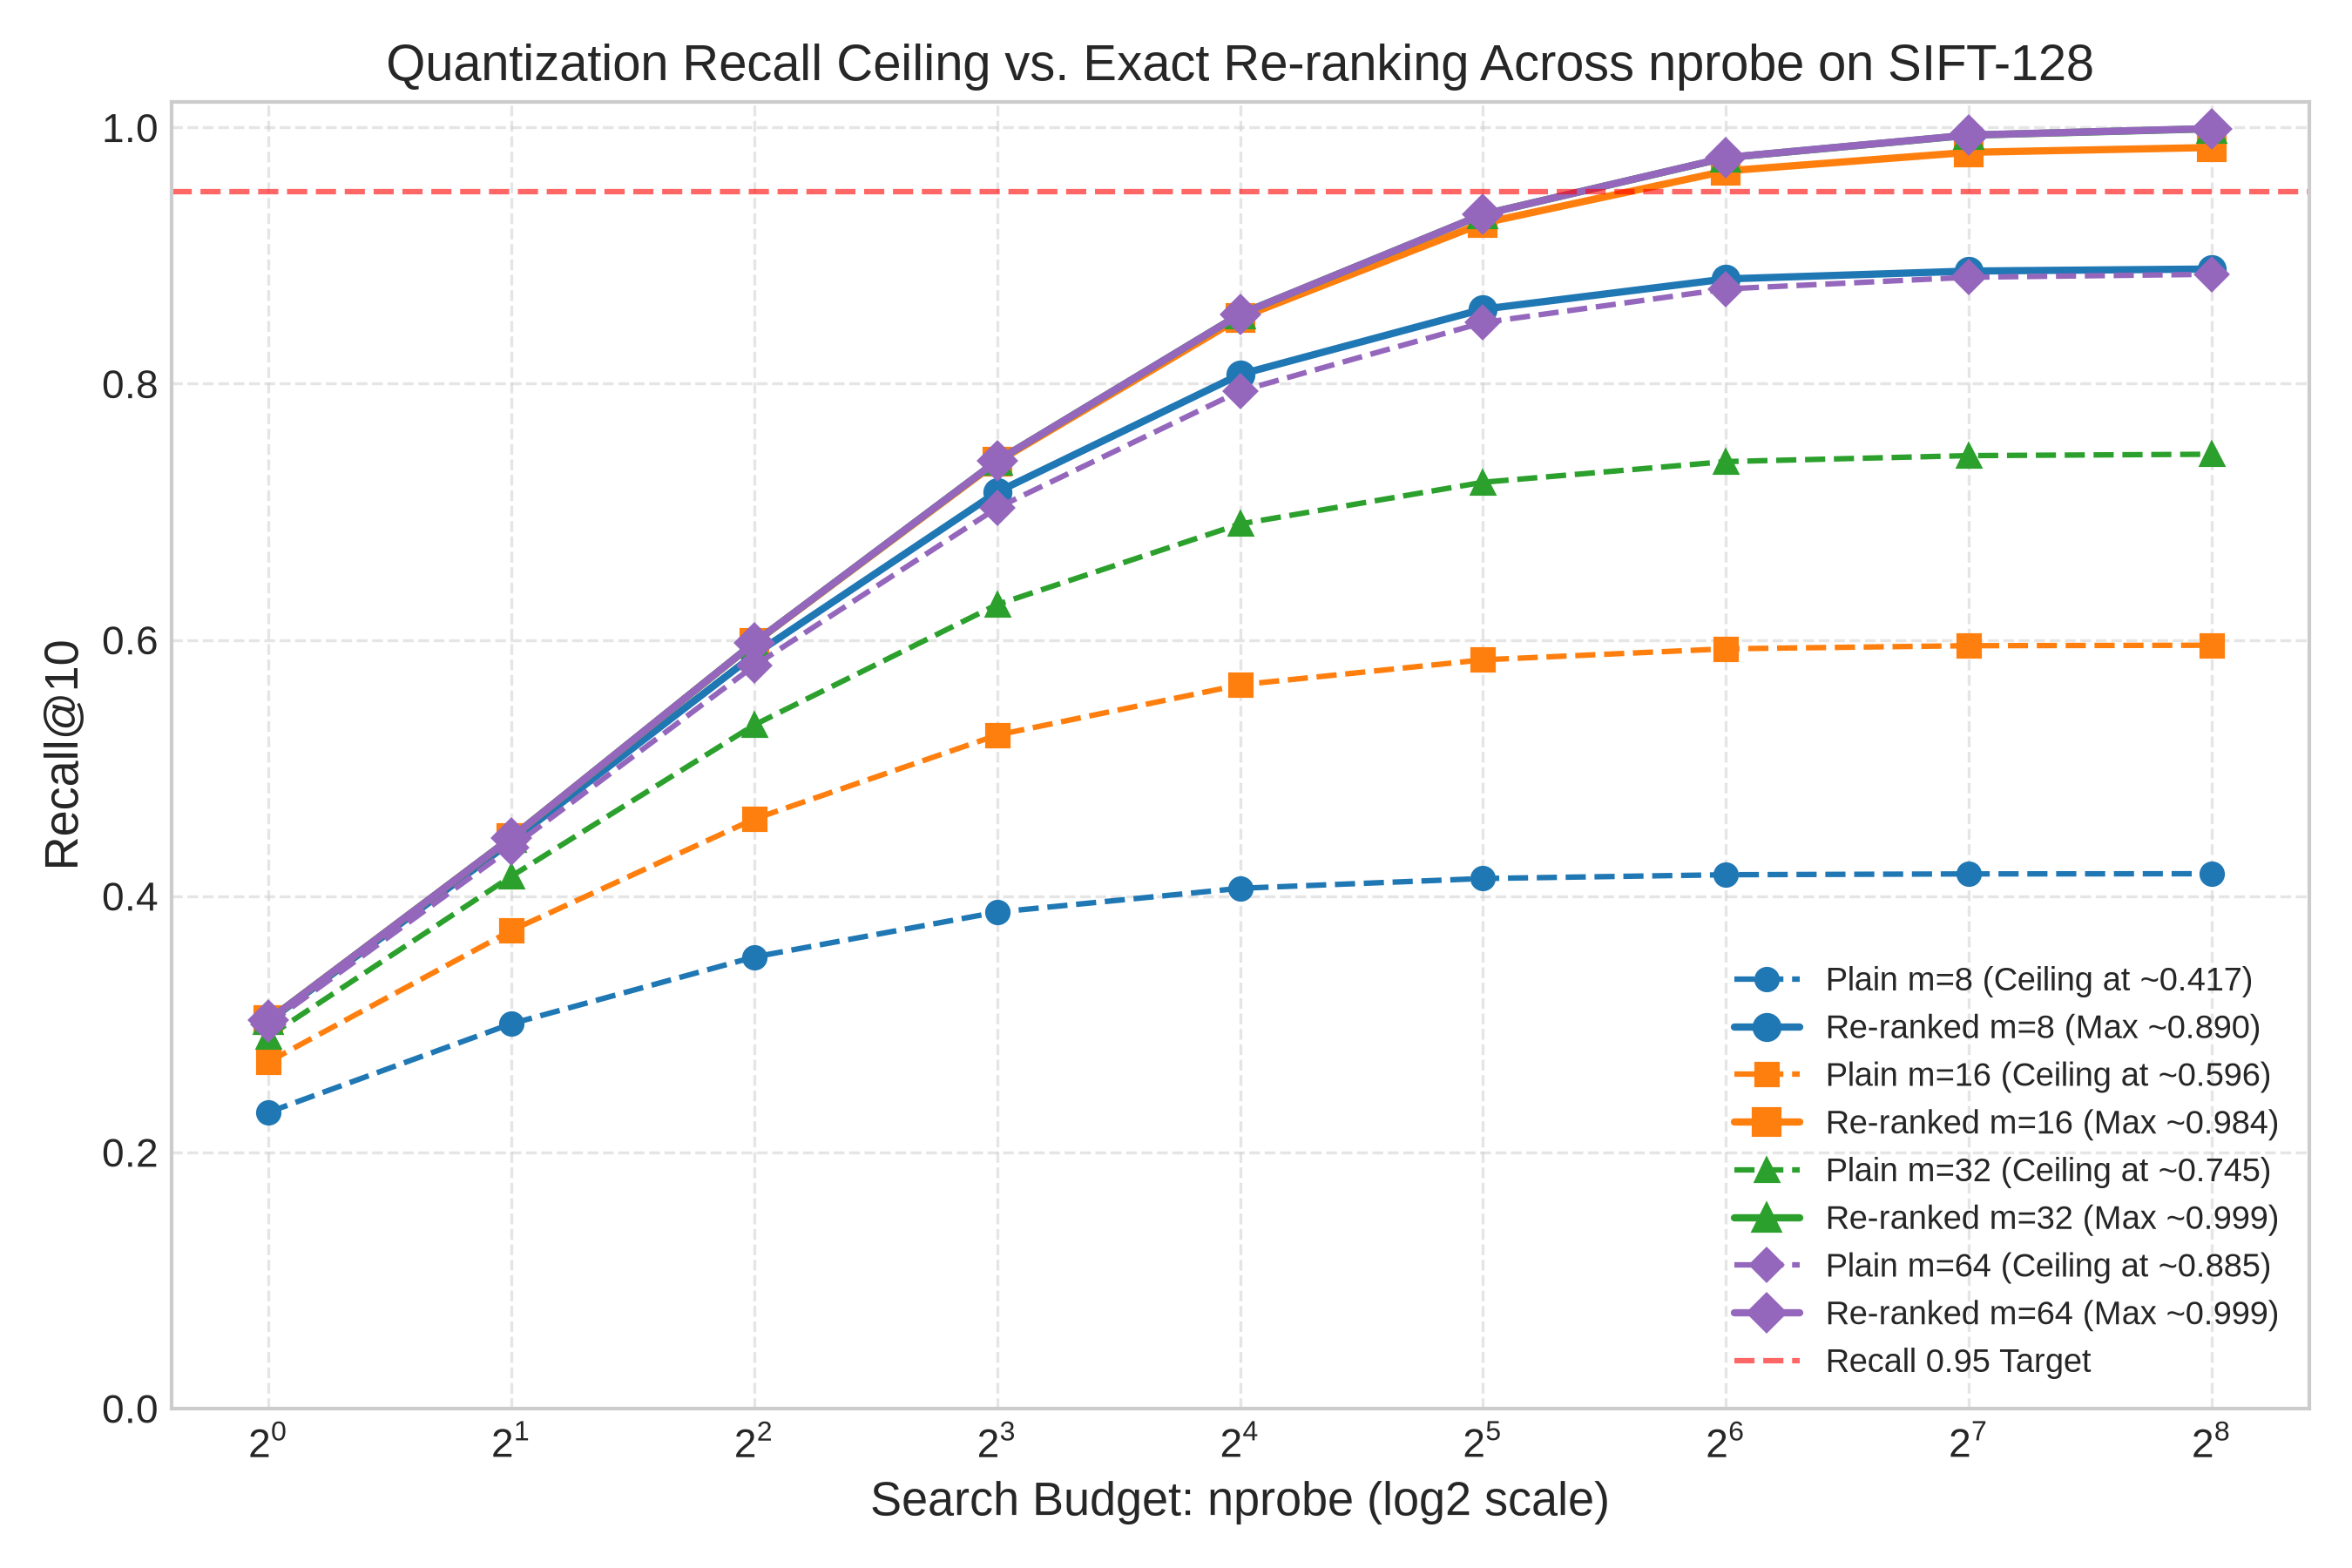
\includegraphics[width=\linewidth, height=3.6cm]{part3_compression_recall_ceiling.png}
        \caption{Quantization recall ceiling vs. exact re-ranking}
        \label{fig:part3_ceiling}
    \end{subfigure}
    \caption{Part 3 Compression Experiment: Plain IVF-PQ vs. Re-ranked IVF-PQ (top 100 candidates) across sub-vector counts $m \in \{8, 16, 32, 64\}$ on SIFT-128.}
    \label{fig:part3_compression}
\end{figure*}

\subsection{Experimental Formulation}
We varied the number of PQ sub-vectors $m \in \{8, 16, 32, 64\}$ (sub-vector dimensions $d' \in \{16, 8, 4, 2\}$) under an inverted file index ($nlist=4096, nbits=8$). Note that Part 3 configures $nlist=4096$ (vs. $nlist=2048$ in Part 2) to provide finer Voronoi cell partitioning, thereby cleanly isolating sub-space quantization distortion from coarse Voronoi routing errors. We benchmarked \textbf{Plain IVF-PQ} against \textbf{Re-ranked IVF-PQ} (\texttt{faiss.IndexRefine}), where the top $k_{refine} = 100$ candidate vectors retrieved from the quantized inverted lists are re-ranked using exact $L_2$ distance against full-precision uncompressed vectors.

\subsection{Empirical Findings \& Hypothesis Evaluation}
Figure~\ref{fig:part3_compression} and Table~\ref{tab:part3_results} present the empirical findings:

\begin{table}[t]
\centering
\small
\caption{Compression \& Exact Re-ranking on SIFT-128 (Part 3)}
\label{tab:part3_results}
\resizebox{\columnwidth}{!}{%
\begin{tabular}{lccccc}
\toprule
\textbf{Setting} & \textbf{Plain Size} & \textbf{Plain Max $R$} & \textbf{Refined $R$ ($np=64$)} & \textbf{Refined QPS} & \textbf{$\ge 0.95$?} \\
\midrule
$m=8$  & 17.4 MB (28$\times$) & 0.4138 & 0.8821 & 4,723.3 & No \\
$m=16$ & 24.0 MB (20$\times$) & 0.5958 & \textbf{0.9661} & \textbf{3,664.4} & \textbf{Yes} \\
$m=32$ & 39.3 MB (12$\times$) & 0.7449 & \textbf{0.9765} & 2,556.3 & \textbf{Yes} \\
$m=64$ & 69.8 MB (7$\times$)  & 0.8854 & \textbf{0.9765} & 1,543.8 & \textbf{Yes} \\
\bottomrule
\end{tabular}%
}
\end{table}

\begin{enumerate}
    \item \textbf{Hypothesis 1 (Ceiling vs. $m$) --- Confirmed}: Plain IVF-PQ exhibited strict asymptotic ceilings: $0.4138$ ($m=8$), $0.5958$ ($m=16$), $0.7449$ ($m=32$), and $0.8854$ ($m=64$). Even with $m=64$ ($d'=2$), plain IVF-PQ fails to reach 0.90 recall.
    \item \textbf{Hypothesis 2 (Restoration via Re-ranking) --- Confirmed}: Re-ranking the top 100 candidates eliminated candidate rank distortion, lifting recall from $0.5930 \to \mathbf{0.9661}$ at $nprobe=64$ for $m=16$ ($+37.3\%$ gain) and reaching $0.999$ for $m=32, 64$. For $m=8$, recall jumped by $+47.6\%$ ($0.4138 \to 0.8899$), but capped below $0.95$ because coarse 16-d sub-vectors displace true 10-NNs outside the top 100 candidate pool.
    \item \textbf{Hypothesis 3 (QPS Overhead) --- Confirmed}: Re-ranking 100 candidates requires $100 \times 128 \approx 12,800$ FLOPs ($<0.05$ ms), retaining \textbf{85.1\% to 99.5\%} of plain QPS at $nprobe \ge 32$. At $0.9661$ recall, Re-ranked IVF-PQ ($m=16$) achieves \textbf{3,664.4 QPS}---$87\times$ faster than exact search and $1.81\times$ faster than IVF-Flat ($2,030.0$ QPS).
    \item \textbf{Hypothesis 4 (Memory Trade-off) --- Confirmed}: Plain IVF-PQ compresses the index to 18.3--73.2 B/vec ($7\times$--$28\times$ reduction). Exact re-ranking requires retaining the uncompressed vectors (512 MB, 512 B/vec), proving that re-ranking restores recall by trading away pure in-memory compression.
\end{enumerate}

\section{Custom Data Experiment: Geometric Cluster Dispersion Failure Mode (Part 4)}
To investigate index failure modes under controlled geometric transformations, we built a synthetic Gaussian Mixture Model (GMM) generator (\texttt{src/generate\_synthetic\_data.py}) and pre-registered our hypotheses in git (\texttt{commit f5c67f3}).

\subsection{Experimental Design}
We generated $N = 200,000$ base vectors in $D = 64$ dimensions with $K = 50$ true cluster centroids on a sphere of radius 3.0, and 2,000 test queries sampled from the same mixture (`seed=42`). We varied \textbf{exactly one property: the intra-cluster standard deviation $\sigma$}:
\begin{itemize}
    \item \textbf{Control ($\sigma = 0.05$)}: Tight, isolated natural clusters.
    \item \textbf{Setting 1 ($\sigma = 0.15$)}: Moderately compact clusters with mild contact.
    \item \textbf{Setting 2 ($\sigma = 0.35$)}: Diffuse clusters with substantial overlap.
    \item \textbf{Setting 3 ($\sigma = 0.70$)}: Ambient noise; clusters completely dissolve.
\end{itemize}
We benchmarked IVF-Flat ($nlist=1024, nprobe \in [1, 128]$) and HNSW ($M=16, efC=64, efSearch \in [10, 320]$).

\begin{figure*}[t]
    \centering
    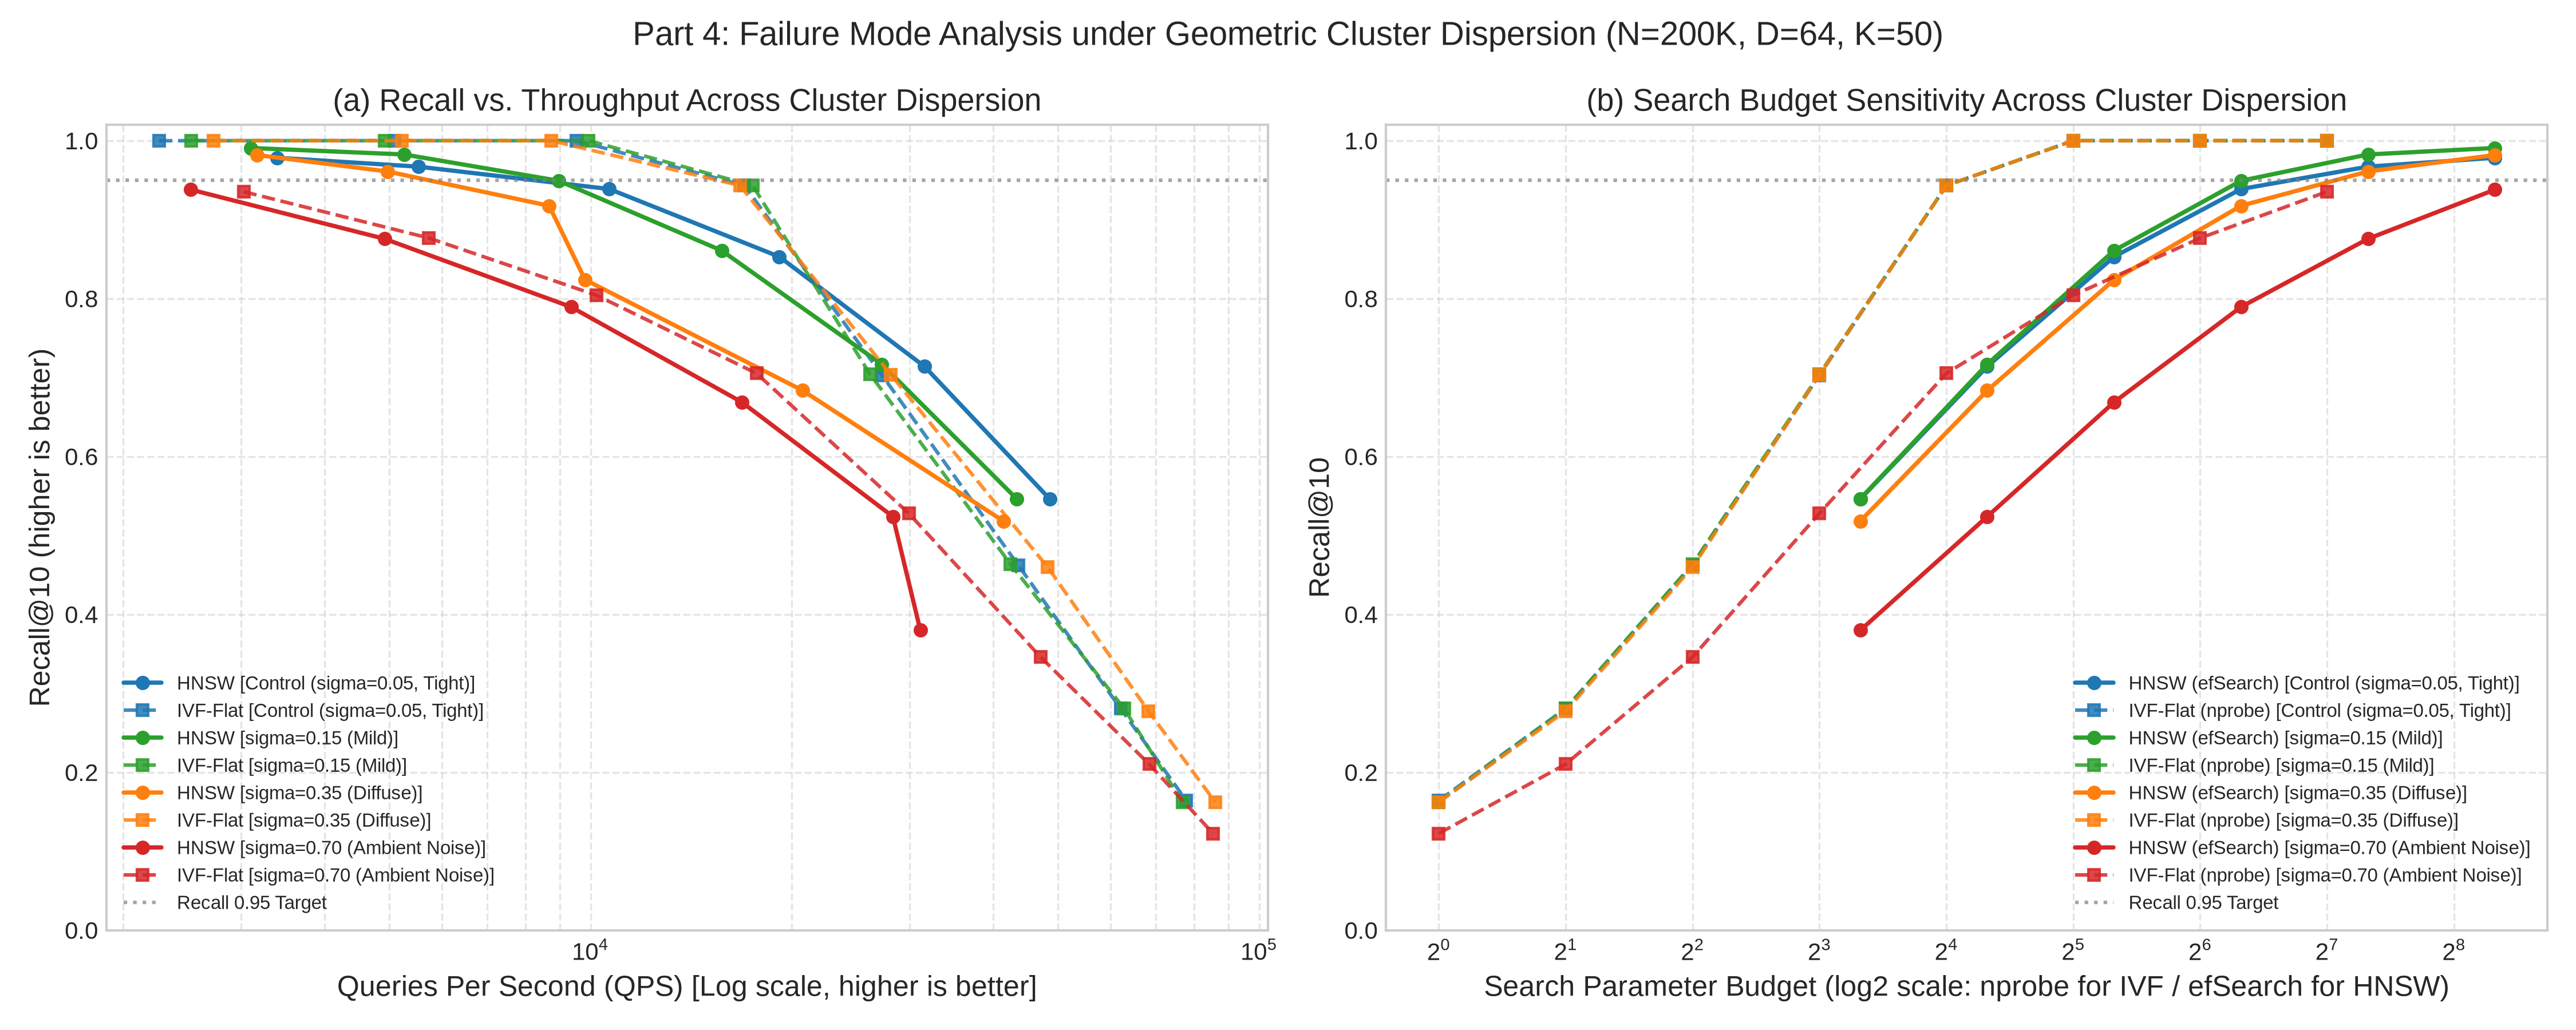
\includegraphics[width=0.92\textwidth, height=3.5cm]{part4_geometry_failure.png}
    \caption{Part 4 Failure Mode Analysis: (a) Recall@10 vs. Throughput and (b) Search budget sensitivity across cluster dispersion $\sigma \in \{0.05, 0.15, 0.35, 0.70\}$ on synthetic data ($N=200\text{K}, D=64, K=50$).}
    \label{fig:part4_failure}
\end{figure*}

\subsection{Empirical Findings \& Mechanisms}
Figure~\ref{fig:part4_failure}, Figure~\ref{fig:part4_dispersion}, and Table~\ref{tab:part4_results} illustrate the failure mechanisms.

\begin{table}[t]
\centering
\small
\caption{Cluster Dispersion Performance on Synthetic Geometry (Part 4)}
\label{tab:part4_results}
\resizebox{\columnwidth}{!}{%
\begin{tabular}{lcccccc}
\toprule
\textbf{Setting} & \textbf{IVF Build} & \textbf{IVF $R$ ($np=16$)} & \textbf{IVF Max $R$} & \textbf{HNSW Build} & \textbf{HNSW Max $R$} & \textbf{$\ge 0.95$?} \\
\midrule
$\sigma = 0.05$ & 4.19s & 0.9432 & 0.9999 & 14.61s & 0.9784 & \textbf{Yes} \\
$\sigma = 0.15$ & 4.17s & 0.9431 & 1.0000 & 14.79s & 0.9907 & \textbf{Yes} \\
$\sigma = 0.35$ & 4.14s & 0.9432 & 1.0000 & 15.21s & 0.9818 & \textbf{Yes} \\
$\sigma = 0.70$ & 4.14s & \textbf{0.7053} & \textbf{0.9354} & \textbf{17.41s} & \textbf{0.9379} & \textbf{FAIL} \\
\bottomrule
\end{tabular}%
}
\end{table}

\begin{figure}[t]
    \centering
    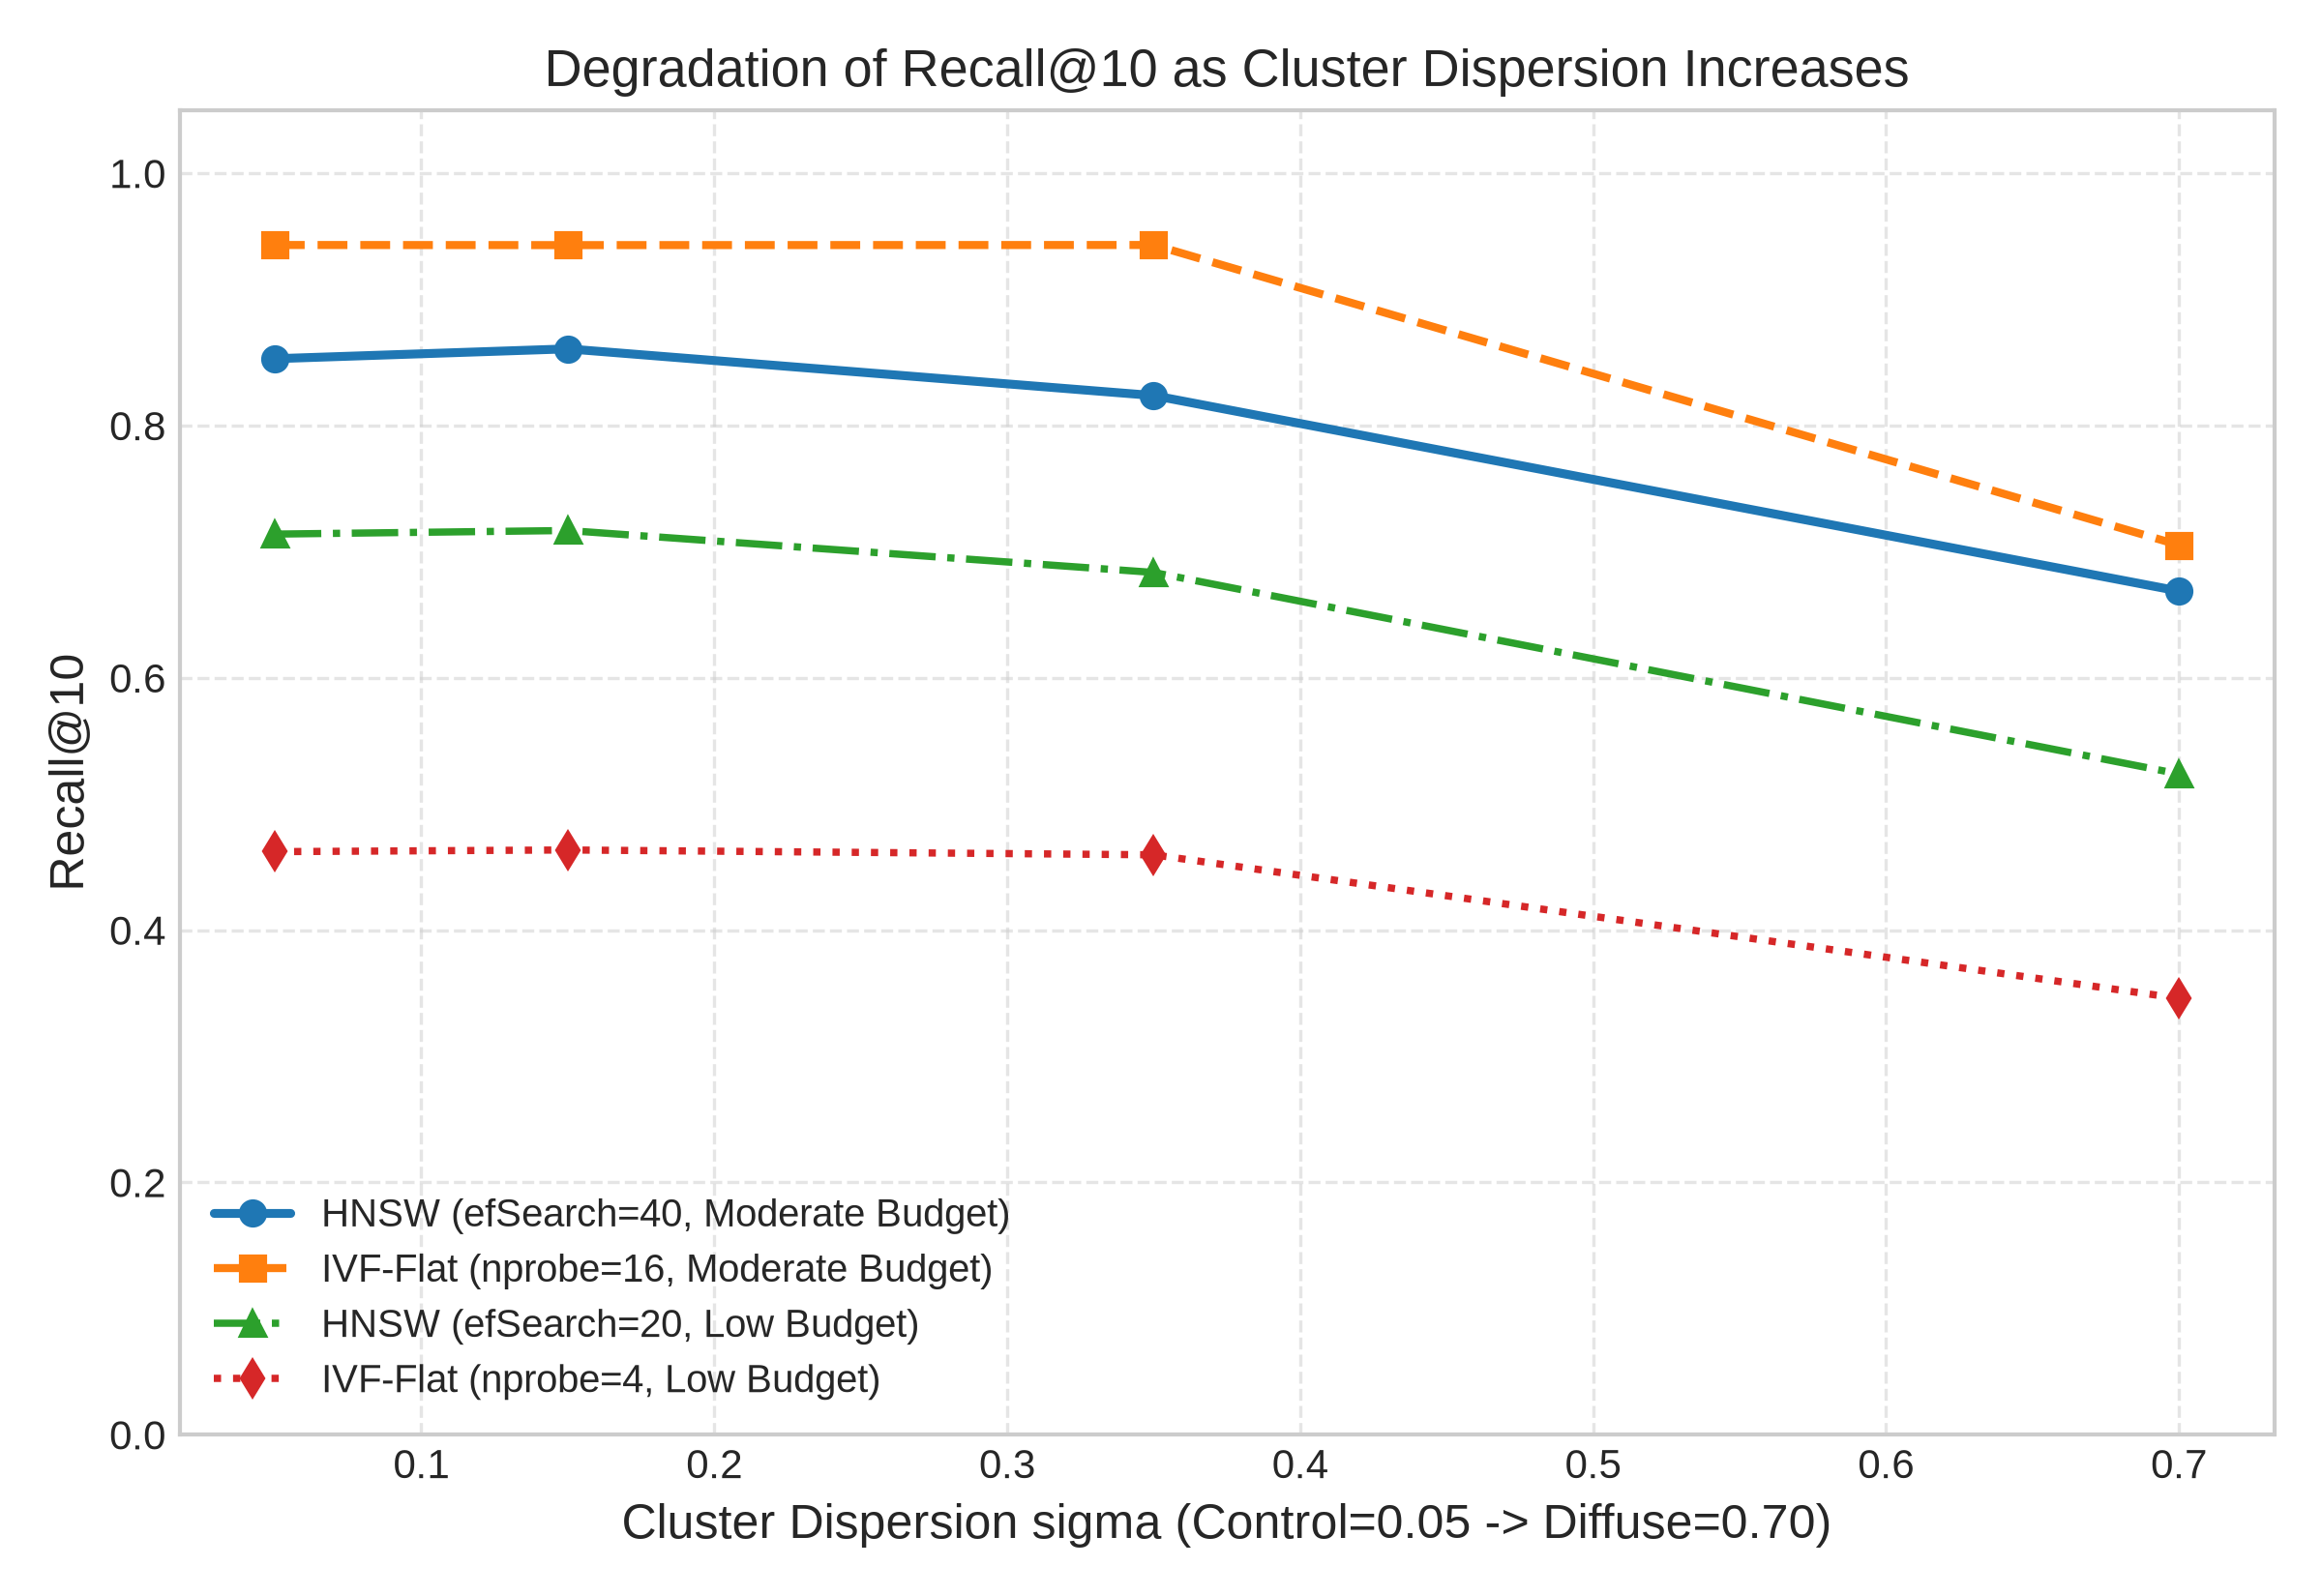
\includegraphics[width=0.75\linewidth, height=2.8cm]{part4_dispersion_impact.png}
    \caption{Direct degradation of Recall@10 as cluster dispersion $\sigma$ increases from 0.05 to 0.70 across fixed search budgets.}
    \label{fig:part4_dispersion}
\end{figure}

\begin{enumerate}
    \item \textbf{Voronoi Boundary Scattering in IVF-Flat}: At $\sigma \le 0.35$, IVF-Flat achieves 100\% recall at $nprobe=32$ ($9,402$ QPS). At $\sigma=0.70$, recall at $nprobe=16$ plummets from $0.9432 \to \mathbf{0.7053}$ ($-23.8\%$), and peaks at $0.9354$ ($nprobe=128$), failing the 0.95 target. \textit{Mechanism}: $k$-means Voronoi partitioning assumes local density concentration. When intra-cluster variance exceeds inter-centroid spacing, true nearest neighbours cross cell boundaries and scatter across dozens of inverted lists.
    \item \textbf{Distance Concentration in HNSW}: At $\sigma=0.70$, HNSW recall at $efSearch=40$ collapses from $0.8608 \to \mathbf{0.6688}$, and caps at $0.9379$ ($efSearch=320$), also failing the 0.95 target. \textit{Mechanism}: Extreme dispersion causes distance concentration ($\frac{D_{10}-D_1}{D_1} \to 0$). Greedy routing on the proximity graph loses downhill directional signal, getting trapped in sub-optimal local minima.
    \item \textbf{Isolated Clique Trapping at $\sigma=0.05$}: At extreme tightness ($\sigma=0.05$), HNSW peak recall ($0.9784$) is lower than under mild dispersion $\sigma=0.15$ ($0.9907$). Tight, distant clusters cause HNSW to form dense intra-cluster cliques with sparse cross-cluster highways, impeding inter-cluster transitions.
    \item \textbf{Resource Scaling}: IVF-Flat build time was invariant to dispersion ($\approx 4.1$s), whereas HNSW build time increased by \textbf{+19.2\%} ($14.61\text{s} \to 17.41\text{s}$) because neighbor search during edge pruning must evaluate broader, less concentrated candidate sets.
\end{enumerate}

\section{Synthesis \& System Analysis (Part 5)}

\subsection{Q1: Fastest Index at Recall 0.95 Across Datasets}
At recall 0.95, \textbf{HNSW is the fastest index on both datasets, but its relative advantage changes drastically}:
\begin{itemize}
    \item On \textbf{SIFT-128}: HNSW achieves \textbf{7,457.6 QPS}, outperforming IVF-Flat ($2,030.0$ QPS) by \textbf{3.67$\times$} and exact search ($42.2$ QPS) by \textbf{177$\times$}.
    \item On \textbf{GloVe-100}: HNSW achieves \textbf{446.0 QPS}, outperforming IVF-Flat ($359.2$ QPS) by only \textbf{1.24$\times$} and exact search ($45.7$ QPS) by \textbf{9.8$\times$}.
\end{itemize}
\textbf{The Geometric Mechanism}: SIFT descriptors represent local visual gradients with low intrinsic dimensionality clustered around visual primitives. HNSW's upper-layer highway edges navigate between clusters in $\mathcal{O}(\log N)$ hops, entering the target cluster near the query. In contrast, GloVe word embeddings populate a dense, high-dimensional spherical shell with severe \textbf{hubness}---certain hub words (e.g., common syntactic words) appear among the nearest neighbours of thousands of queries. Hub nodes create high graph in-degrees that distort greedy routing, forcing HNSW to expand deep search buffers ($efSearch \ge 800$) to circumvent hubs, eroding its speed advantage over inverted list scanning.

\subsection{Q2: Build Time, Memory Costs, and the PQ Trade-off}
\textbf{Build Time}: Exact search requires zero indexing time (0.2s array allocation). IVF-Flat builds rapidly (34--38s for $\sim 1\text{M}$ vectors) via mini-batch $k$-means. HNSW requires extensive neighbor selection and edge pruning, taking $130.6$s on SIFT and $208.3$s on GloVe ($3.5\times$--$6\times$ slower than IVF-Flat).

\textbf{Memory Footprint}: IVF-Flat incurs minimal overhead over raw vectors (497 MB on SIFT = 521 B/vec vs. 512 B/vec raw). HNSW adds bidirectional graph adjacency lists ($2 \times M \times 4$ bytes per link), consuming 748 MB (784 B/vec, $+53\%$ overhead). 

\textbf{What PQ Saves and Gives Up}: 
\begin{itemize}
    \item \textbf{What it saves}: IVF-PQ compresses the index to 70.8 MB on SIFT (74.3 B/vec) and 66.4 MB on GloVe (58.8 B/vec), achieving \textbf{$7\times$ to $28\times$ memory reduction}.
    \item \textbf{What it gives up}: PQ surrenders continuous distance resolution. Sub-space quantization distortion creates rank scrambling that imposes an impassable recall ceiling (0.885 on SIFT, 0.829 on GloVe). To reach 0.95 recall, PQ requires exact re-ranking, which restores recall but forces the system to store uncompressed vectors (512 MB), nullifying in-memory compression.
\end{itemize}

\subsection{Q3: Implications of Parts 3 and 4 on Headline Numbers}
Public benchmark leaderboards (e.g., ann-benchmarks) report peak QPS under ideal clustered geometries and static in-distribution queries. Our findings demonstrate two critical failure modes where headline numbers mislead:
\begin{enumerate}
    \item \textbf{The Incomplete Metric Trap (Part 3)}: Leaderboards often highlight plain IVF-PQ's 20,000+ QPS and tiny memory footprint. However, because plain PQ cannot exceed 0.88 recall, headline QPS figures are unusable for production retrieval systems requiring $R \ge 0.95$. Exact re-ranking achieves 0.966 recall at 3,664 QPS, but requires $7\times$ more memory than advertised.
    \item \textbf{The Geometry Mismatch Trap (Part 4)}: When data geometry deviates from tight cluster manifolds (as shown in Part 4 at $\sigma=0.70$), both IVF-Flat and HNSW fail to reach 0.95 recall. In systems with diffuse embeddings or out-of-distribution queries, real-world throughput will collapse compared to leaderboard claims.
\end{enumerate}

\subsection{Q4: Deployment Recommendation (150K vs. 10M Vectors)}
\textbf{Constraints}: 100 ms query SLA, 16 GB RAM budget.
\begin{itemize}
    \item \textbf{Scale 1: $N = 150,000$ Vectors ($D=128$, float32)}: Storing 150K vectors requires $150\text{K} \times 128 \times 4\text{ B} \approx \mathbf{76.8\text{ MB}}$ ($<0.5\%$ of 16 GB). Scaling from our 1M SIFT benchmark (23.72 ms), exact single-thread search takes $\frac{150\text{K}}{1\text{M}} \times 23.72\text{ ms} = \mathbf{3.56\text{ ms}}$ ($<0.5$ ms in batch), well inside the 100 ms SLA. \textbf{Recommendation}: \textbf{Use Exact Brute-Force Search (\texttt{IndexFlatL2})}. Exact search delivers 100\% recall with zero index build time, zero tuning, and minimal memory. Using ANN introduces unnecessary complexity and recall loss.
    \item \textbf{Scale 2: $N = 10,000,000$ Vectors ($D=128$, float32)}: Exhaustive search takes $\frac{10\text{M}}{1\text{M}} \times 23.72\text{ ms} \approx 237.2\text{ ms}$, violating the 100 ms SLA; ANN is mandatory. HNSW ($M=32$) requires $\approx 7.84\text{ GB}$ and takes $\sim 25$ min to build, leaving limited RAM headroom for concurrency. \textbf{Recommendation}: \textbf{IVF-Flat ($nlist=16384, nprobe=64$)} or \textbf{Re-ranked IVF-PQ ($nlist=16384, m=16, k_{refine}=100$)}. IVF-Flat requires $5.21\text{ GB}$ RAM, builds in $\sim 6$ min, and delivers $\approx 200$ QPS (5 ms latency) at $R \ge 0.95$. If RAM must be shared, Re-ranked IVF-PQ keeps 250 MB PQ codes in RAM while memory-mapping raw vectors from NVMe SSD, achieving $<2$ ms latency.
\end{itemize}

\subsection{Q5: Two Ways Our Benchmark Could Be Misleading}
\begin{enumerate}
    \item \textbf{Single-Query Sequential Timing vs. Concurrent Workloads}: Our benchmark measures queries sequentially on a single thread with warm caches. In production, multi-threaded servers face memory bus contention and cache thrashing. \textbf{We tested this}: In Part 1, single-query vs. batch execution revealed a $7.4\times$ throughput divergence due to memory bandwidth saturation and cache amortization.
    \item \textbf{Static Read-Only Indexes vs. Dynamic Streaming Updates}: Our benchmark evaluates static indexes from fixed distributions. Production systems experience continuous insertions, updates, and deletions, which degrade HNSW graph connectivity and cause IVF centroids to drift. \textbf{We did not test dynamic updates}, making this an important direction for future benchmarking.
\end{enumerate}

\section{Conclusion}
This work systematically benchmarked exact search, HNSW, IVF-Flat, and IVF-PQ across visual descriptors, word embeddings, and controlled synthetic manifolds. We demonstrated that HNSW's throughput advantage is heavily governed by data geometry (shrinking from $3.67\times$ on SIFT to $1.24\times$ on GloVe). We resolved IVF-PQ's recall ceiling via candidate re-ranking (reaching 0.966 recall at 3,664 QPS), and proved that extreme cluster dispersion causes Voronoi boundary scattering in space-partitioning structures.

\end{document}